\def\MyCourse{データサイエンスコース}
\def\MySubject{R入門}
\def\MySemester{春学期}

\newcommand{\R}{\textbf{R}}
\newcommand{\RStudio}{\textbf{RStudio}}
\newcommand{\Excel}{\textbf{Excel}}
\newcommand{\cs}[1]{\textcolor{blue}{\texttt{#1}}} % Console prompt >


\subsection{観測データと試験データの作成}

\myffr

  \mybfr{手順}
    観測値,時刻データ(1--20),予測対象時刻データ(21--30),
    全期間時刻データ(1--30)を作成する.\\
    現実的には,真値は分からないがこれも作成する.
  \mybto

  \myefr{コンソール}
    \myon{1,7}
    \cs{n.obs <- 20; n.fct <- 10; n.all <- n.obs + n.fct} \hfill \mycheck{データサイズ}\\
    \myon{2,7}
    \cs{x.obs <- 1:n.obs; x.all <- 1:n.all}      \hfill \mycheck{観測時刻;全時刻}\\
    \myon{3,7}
    \cs{f <- function(x) 1 + x + x \^ \ 2}       \hfill \mycheck{真のモデル}\\
    \myon{4,7}
    \cs{e <- rnorm(n = n.obs, sd = 30)}          \hfill \mycheck{観測ノイズ}\\
    \myon{5,7}
    \cs{y.obs~ <- f(x.obs) + e}                  \hfill \mycheck{観測値}\\
    \myon{6,7}
    \cs{y.true <- f(x.all)}                      \hfill \mycheck{真値}
    \myon{7}

  \myeto

  \mybfr{演習}
    どのような値が入っているか確認してください.
  \mybto
  
\end{frame}

\subsection{学習(フィッティング)}

\myffr

  \mybfr{手順}
    lm関数を用いて線形モデルのフィッティングを行う.
    変数の加工は\texttt{I()}で囲む.切片は標準でモデルに入っている.
  \mybto

  \myefr{コンソール}
  \cs{fit <- lm('y \~\ x + I(x\^\relax 2)', data=data.frame(x=x.obs, y=y.obs))}\\
  \cs{summary(fit)}\\
    \vspace{-5mm}
\begin{verbatim}
             Estimate Std. Error t value Pr(>|t|)
 (Intercept)   1.8203    25.8913   0.070    0.945
 x            -4.7082     5.6784  -0.829    0.419
 I(x^2)        1.3641     0.2627   5.194 7.32e-05 ***
\end{verbatim}
    \vspace{-3mm}
  \myeto

  \mycheck{\texttt{Estimate}: 回帰係数推定値},\mycheck{\texttt{Pr(>|t|)}: p値(星屑が付いていれば有意)}

  \mybfr{演習}
    モデル y \~ \ x + I(x \^ \ 2) を変えて,フィッティングしてください.
  \mybto
  
\end{frame}

\subsection{予測}

\myffr

  \mybfr{手順}
    predict関数(正式名:predict.lm)を用いて未来予測を行う.
  \mybto

  \myefr{コンソール}
    \cs{m <- predict(fit, newdata = data.frame(x = x.all),\\
    \hfill interval = 'prediction', level = 0.95)} \\
    \cs{tail(m, 2)}
    \vspace{-5mm}
      \begin{verbatim}
              fit      lwr      upr
      29 1012.4739 818.1671 1206.781
      30 1088.2464 874.4287 1302.064
      \end{verbatim}
    \vspace{-8mm}
  \myeto

  \mycheck{interval: 区間推定種類,level: 信頼水準}\\
  \mycheck{fit:予測値,lwr:下限値,upr:上限値} \mycheck{tail: 末尾データ閲覧関数(cf. head)}

  \mybfr{演習}
   区間の種類(信頼区間:confidence,予測区間:prediction)や信頼水準(level)を変えて値がどう変化するか確認してください.
  \mybto
  
\end{frame}

\subsection{回帰モデルグラフ}

\myffr

\begin{minipage}{0.50\hsize}
\tiny
\vspace{-3mm}
\lstinputlisting[language=R, firstline=3,lastline=28]{061-lm-plot.r}
\vspace{-4mm}
\normalsize
\end{minipage}
\begin{minipage}{0.45\hsize}

\begin{figure}[t]
  \centering
  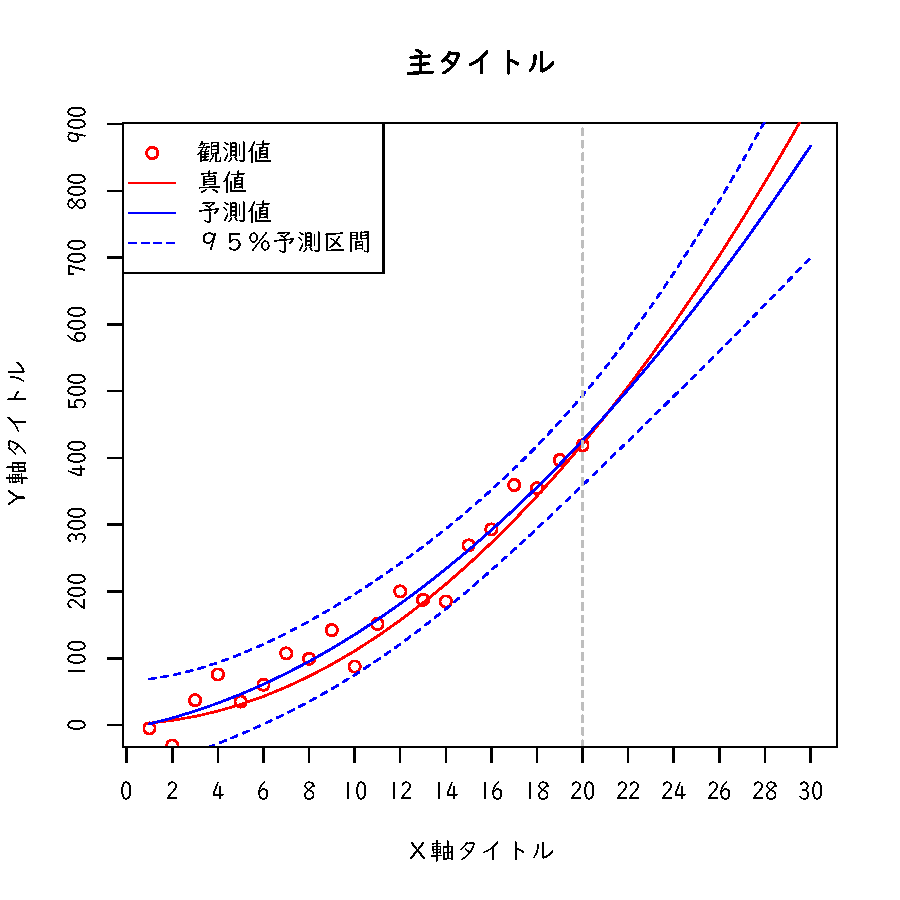
\includegraphics[width=\hsize]{fig/lm}
  \caption{回帰モデルグラフ描画例}
  \label{fig:lm60}
\end{figure}
\vspace{-8mm}
\mycheck{描画関数\tiny{matpoints: 点,matlines: 線,abline: 縦横線,axis: 軸,legend: 凡例}}\\
\mycheck{描画オプション\tiny{col: 色,pch: 点種,lty: 線種,v:縦線,h:横線}}

\end{minipage}

\end{frame}

\end{document}

